
% v2-acmsmall-sample.tex, dated March 6 2012
% This is a sample file for ACM small trim journals
%
% Compilation using 'acmsmall.cls' - version 1.3 (March 2012), Aptara Inc.
% (c) 2010 Association for Computing Machinery (ACM)
%
% Questions/Suggestions/Feedback should be addressed to => "acmtexsupport@aptaracorp.com".
% Users can also go through the FAQs available on the journal's submission webpage.
%
% Steps to compile: latex, bibtex, latex latex
%
% For tracking purposes => this is v1.3 - March 2012
\documentclass[prodmode,acmtecs]{acmsmall} % Aptara syntax
\usepackage[spanish,polish]{babel}
\usepackage[T1]{fontenc}
\usepackage{fancyvrb}
\usepackage{graphicx,hyperref}
\newcommand\cutout[1]{}


\usepackage[table]{xcolor}
\usepackage[utf8]{inputenc}
\usepackage[parfill]{parskip}
\usepackage{tabulary}
\PassOptionsToPackage{hyphens}{url}
\usepackage{hyperref}    
\usepackage[capitalize]{cleveref}


% Metadata Information
% !!! TODO: SET THESE VALUES !!!
\acmVolume{0}
\acmNumber{0}
\acmArticle{CFP}
\acmYear{0}
\acmMonth{0}

\newcounter{colstart}
\setcounter{page}{4}

\RecustomVerbatimCommand{\VerbatimInput}{VerbatimInput}%
{
%fontsize=\footnotesize,
fontfamily=\rmdefault
}


\newcommand{\UnderscoreCommands}{%\do\verbatiminput%
\do\citeNP \do\citeA \do\citeANP \do\citeN \do\shortcite%
\do\shortciteNP \do\shortciteA \do\shortciteANP \do\shortciteN%
\do\citeyear \do\citeyearNP%
}

\usepackage[strings]{underscore}



% Document starts
\begin{document}


\setcounter{colstart}{\thepage}

\acmArticle{CFP}
\title{\huge\sc SIGLOG Monthly 214}
\author{DAVID PURSER\affil{Max Planck Institute for Software Systems, Saarbr\"ucken}
\vspace*{-2.6cm}\begin{flushright}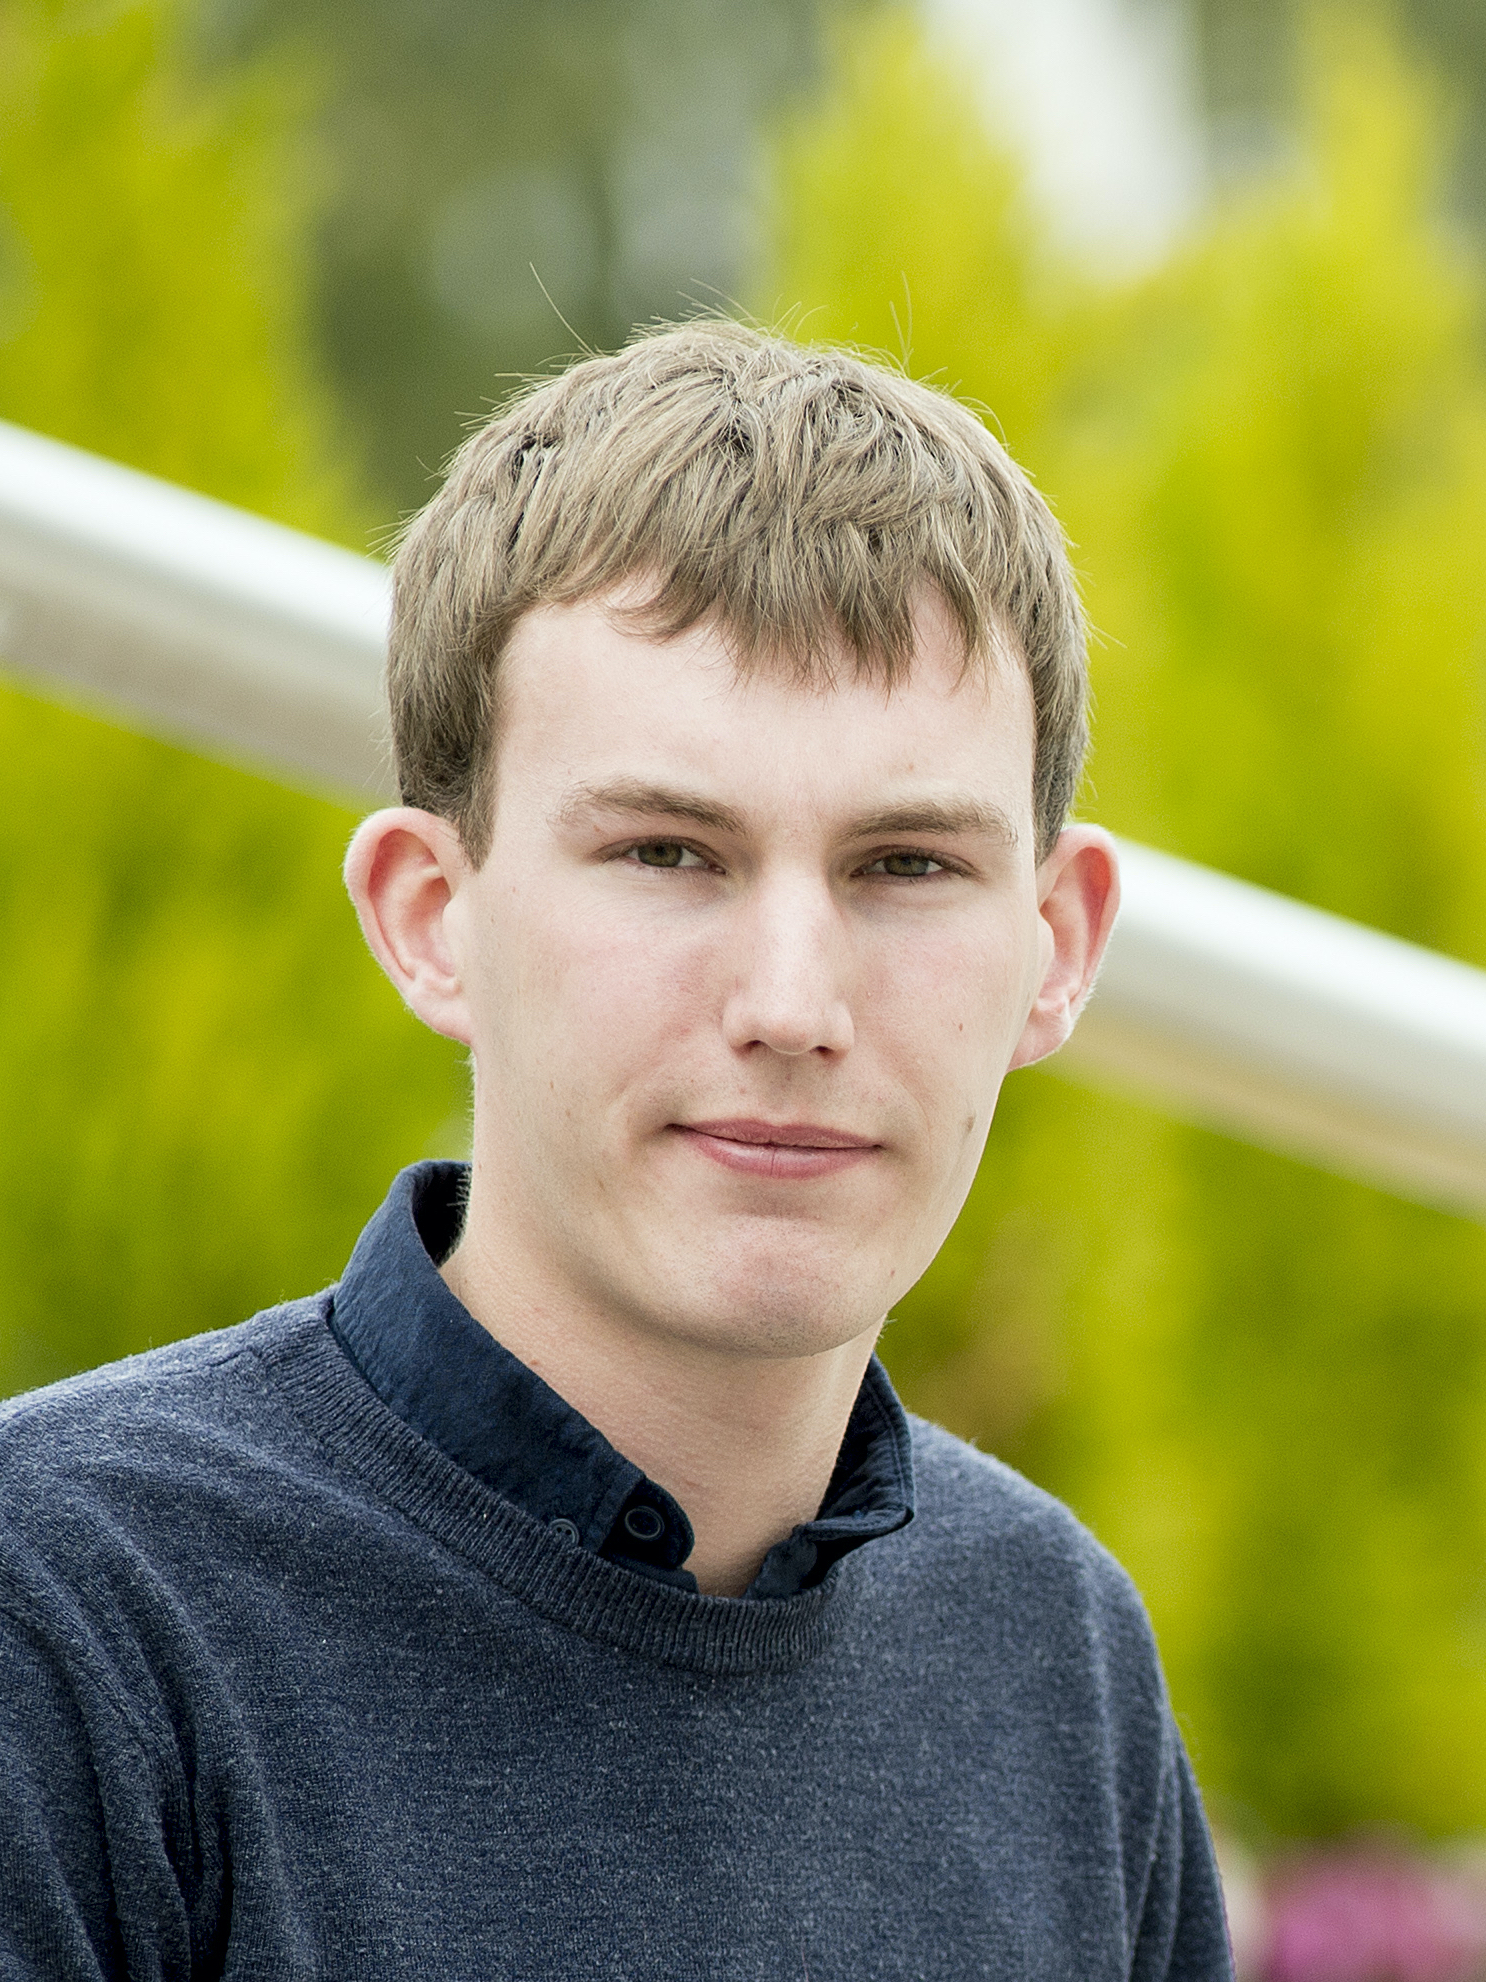
\includegraphics[width=30mm]{dp}\end{flushright}
}

\maketitlee

\href{https://lics.siglog.org/newsletters/}{Past Issues}
 - 
\href{https://lics.siglog.org/newsletters/inst.html}{How to submit an announcement}
\section{Table of Content}\begin{itemize}\item DEADLINES (\cref{deadlines}) 
 
\item SIGLOG MATTERS 
 
\begin{itemize}\item The 2021 Alonzo Church Award for Outstanding Contributions to Logic and Computation (\cref{The2021AlonzoChurchAwardforOutstandingContributionstoLogicandComputation})
\end{itemize} 
\item CALLS 
 
\begin{itemize}\item FVPS 2021 (CALL FOR PAPERS) (\cref{FVPS2021})
\item ICGT 2021 (CALL FOR REGISTRATION) (\cref{ICGT2021})
\item ICALP 2023 (CALL FOR LOCATION) (\cref{ICALP2023})
\item CPSIoTSec 2021 (CALL FOR PAPERS) (\cref{CPSIoTSec2021})
\item CiE 2021 (CALL FOR PARTICIPATION) (\cref{CiE2021})
\item RW 2021 (CALL FOR PARTICIPATION) (\cref{RW2021})
\item OVERLAY 2021 (CALL FOR CONTRIBUTIONS) (\cref{OVERLAY2021})
\item CCC 2021 (CALL FOR SUBMISSIONS) (\cref{CCC2021})
\end{itemize} 
\item JOB ANNOUNCEMENTS 
 
\begin{itemize}\item MPI for Informatics in Saarbrücken (PhD Position) (\cref{MPIforInformaticsinSaarbrckenPhDPosition})
\end{itemize} 
\end{itemize}\section{Deadlines}\label{deadlines}\rowcolors{1}{white}{gray!25}\begin{tabulary}{\linewidth}{LL}HIGHLIGHTS 2021:  & Jun 04, 2021 (Submission deadline (7pm GMT)) \\
ICGI 2020/21:  & Jun 06, 2021 (Paper, EXTENDED) \\
CALCO 2021:  & Jun 10, 2021 (Paper, EXTENDED) \\
PODS 2022:  & Jun 11, 2021 (First cycle abstract), Jun 18, 2021 (Full paper) \\
FVPS 2021:  & Jun 11, 2021 (Full Paper) \\
ICGT 2021:  & Jun 12, 2021 (Early registration) \\
ESSLLI 2022:  & Jun 15, 2021 (Course Title), Jun 22, 2021 (Final) \\
ICALP 2023:  & Jun 15, 2021 (The deadline for proposals) \\
EXPRESS/SOS 2021:  & Jun 21, 2021 (Paper) \\
NMR-2021:  & Jun 25, 2021 (Paper registration), Jun 30, 2021 (Paper) \\
CPSIoTSec 2021:  & Jun 25, 2021 (Submission deadline), Jul 30, 2021 (Submission deadline only for papers rejected from ACM CCS 2021) \\
ACKERMANN AWARD 2021:  & Jul 01, 2021 (Deadline for nomination) \\
CSL22:  & Jul 05, 2021 (Abstract), Jul 12, 2021 (Paper) \\
OVERLAY 2021:  & Jul 11, 2021 (Paper) \\
RW 2021:  & Aug 25, 2021 (Registration closes) \\
CCC 2021:  & Aug 30, 2021 (Deadline) \\
\end{tabulary}
\section{The 2021 Alonzo Church Award for Outstanding Contributions to Logic and Computation}\label{The2021AlonzoChurchAwardforOutstandingContributionstoLogicandComputation}ANNOUNCEMENT 

\begin{itemize}\item  The ACM Special Interest Group on Logic (SIGLOG), the European Association for Theoretical Computer Science (EATCS), the European Association for Computer Science Logic (EACSL), and the Kurt Goedel Society (KGS) are pleased to announce that 
 
  Georg Gottlob, Christoph Koch, Reinhard Pichler, Klaus U. Schulz, and Luc Segoufin 
 
  have been selected as the winners of the 2021 Alonzo Church Award for Outstanding Contributions to Logic and Computation for fundamental work on logic-based web data extraction and querying tree-structured data, published in: 
 
\begin{itemize}\item  (1) Georg Gottlob and Christoph Koch. “Monadic Datalog and the Expressive Power of Lan- guages for Web Information Extraction.” Journal of the ACM (JACM) 51.1 (2004): 74-113.
\item  (2) Georg Gottlob, Christoph Koch, and Klaus U. Schulz. “Conjunctive Queries Over Trees.” Journal of the ACM (JACM) 53.2 (2006): 238-272.
\item  (3) Georg Gottlob, Christoph Koch, and Reinhard Pichler. “Efficient Algorithms for Processing XPath Queries.” ACM Transactions on Database Systems (TODS) 30.2 (2005): 444-491.
\item  (4) Georg Gottlob, Christoph Koch, Reinhard Pichler, and Luc Segoufin. “The Complexity of XPath Query Evaluation and XML Typing.” Journal of the ACM (JACM) 52.2 (2005): 284-335.
\end{itemize} 
\item  THE CONTRIBUTION 
 
\begin{itemize}\item  Paper (1) establishes a comprehensive logical theory of Web data extraction. At its core, this is the problem of selecting relevant nodes (subtrees) from HTML text. While the set of relevant nodes can be expressed in Monadic Second-Order logic (MSO) over finite trees, MSO has high computationally complexity. The authors prove that Monadic Datalog on trees has exactly the same expressive power as full MSO and that, surprisingly, evaluating Monadic Datalog is feasible in time linear in the size of query and input tree. These results greatly influenced theoretical and applied research, and gave rise to logic-based systems for data extraction that have been successfully used in industry.
\item  Papers (2,3,4) present deep investigations into logical queries over tree-structured data. The complexity of evaluating XPath, a key technology in Web browsers and other systems, was unclear, and available implementations required exponential time. Paper (2) gives a full characterization of, and a dichotomy theorem for, the complexity of conjunctive queries on various representations of trees. Paper (3) shows that the full XPath standard can be evaluated in PTIME and proposes a logical core which has become seminal to research efforts at the intersection of Web data processing and (modal) logics. Finally, paper (4) establishes the precise complexity of evaluating XPath fragments.
\end{itemize} 
\end{itemize}\section{FVPS 2021: Workshop on Formal Verification of Physical Systems}\label{FVPS2021}  July 26 - 31, 2021  Timișoara, Romania\\ 
  Co-located with CICM 2021\\ 
  \href{https://cicm-conference.org/2021/cicm.php?event=fvps\&menu=general}{https://cicm-conference.org/2021/cicm.php?event=fvps\&menu=general}\\ 
  \href{https://easychair.org/cfp/FVPS-2021}{https://easychair.org/cfp/FVPS-2021}\\ 
CALL FOR PAPERS 

\begin{itemize}\item  THEME 
 
  One of the main issues behind many failing systems is the ad-hoc verification approach that involves a variety of formalism and techniques for the modeling and analysis of various components of the present-age (cyber)-physical systems. For example, control and communication protocols are usually modeled using automata theory, and thus analyzed using model checking techniques, while the modeling of physical aspects often requires multivariate calculus foundations, which are in turn analyzed using paper-and-pencil based analytical proofs, simulation or theorem proving. The fundamental differences between these modeling and analysis techniques limit us to analyze the whole system as one unit and thus miss many corner cases, which arise due to the operation of all the sub-components of the system together. One of the major concerns is that, despite the above-mentioned evident limitations in the analysis methods, many safety-critical systems, such as aerospace, smart-transportation, smart-grid and e-healthcare, are increasingly involving physical elements. Moreover, we are moving towards integrating more complex physical elements in our engineering systems. For example, we are moving towards Quantum Computers to meet the high-performance needs. Similarly, phonic components are increasingly being advocated and used in aerospace applications due to their lightweight and temperature independency compared to traditional electronics-based components. Finally, the impact of physical components is relevant to both safety and security of the overall system. For example, malfunction in sensor measurement may lead to safety issues whereas sophisticated physics-based side-channel (e.g., power and acoustic measurements) attacks lead to the security violation of the underlying system.  
 
  The focus of the workshop will be on formal verification techniques for the modeling, analysis and verification of safety and security critical physical systems. We encourage submissions on interdisciplinary approaches that bring together formal methods and techniques from other knowledge areas such as quantum computing, control theory, biology, optimization theory and artificial intelligence.  
 
\item  TOPICS OF INTEREST 
 
  Topics of interest include (but are not limited to): 
 
  General Topics 
 
\begin{itemize}\item  Formalization of mathematics and physics theories
\item  Interactive and automated theorem proving for physical systems
\item  Model Checking algorithms and tools for physical systems
\item  Formalization of security and safety of physical systems
\item  Runtime verification of safety and security properties
\item  Combination of formal, semi formal and informal approaches
\item  Formal verification of numerical algorithms
\item  Refinement based verification of physical systems
\item  Formalization of probability, reliability and statistical metrics
\item  Hybrid systems
\item  Benchmarks for physical systems
\item  Formal requirement specification and validation
\end{itemize} 
 Application Domain 
 
\begin{itemize}\item  Aerospace and avionics systems
\item  Automotive cyber physical systems
\item  Robotics
\item  Smart Grids
\item  Smart transportation
\item  Human factor modeling and analysis
\item  Biological and healthcare systems
\end{itemize} 
\item  SUBMISSION  
 
\begin{itemize}\item  Regular papers describing developed work with theoretical results (up to 15 pages)
\item  Short papers on experience reports, tools or work in progress with preliminary results (up to 6 pages)
\end{itemize} 
  Submit PDF in column style of CEUR-WS at \href{https://easychair.org/conferences/?conf=fvps2021}{https://easychair.org/conferences/?conf=fvps2021} 
 
  The submissions will be reviewed by at least three PC members. At least one author of each accepted paper is expected to attend FVPS and present the paper. 
 
\item  IMPORTANT DATES 
 
\rowcolors{1}{white}{gray!25}\begin{tabulary}{\linewidth}{LL}Full Paper submission:  & Jun 11, 2021 \\
Notification:  & Jul 12, 2021 \\
Workshop:  & Jul 26-31, 2021 \\
Camera Ready:  & Aug 13, 2021 \\
\end{tabulary}
 
\end{itemize}\section{ICGT 2021: 14th International Conference on Graph Transformation}\label{ICGT2021}  \href{https://icgt2021.di.unipi.it/}{https://icgt2021.di.unipi.it/}\\ 
  June 24-25 Bergen, Norway, co-located with STAF 2021 (FULLY VIRTUAL)\\ 
CALL FOR REGISTRATION 

\begin{itemize}\item  AIMS AND SCOPE 
 
  The use of graphs and graph-like structures as a formalism for specification and modelling is widespread in all areas of computer science as well as in many fields of computational research and engineering. Relevant examples include software architectures, pointer structures, state space and control/data flow graphs, UML and other domain-specific models, network layouts, topologies of cyber-physical environments, quantum computing and molecular structures. Often, these graphs undergo dynamic change, ranging from reconfiguration and evolution to various kinds of behaviour, all of which may be captured by rule-based graph manipulation. Thus, graphs and graph transformation form a fundamental universal modelling paradigm that serves as a means for formal reasoning and analysis, ranging from the verification of certain properties of interest to the discovery of fundamentally new insights. 
 
  The International Conference on Graph Transformation aims at fostering exchange and collaboration of researchers from different backgrounds working with graphs and graph transformation, either in contributing to their theoretical foundations or by applying established formalisms to classical or novel areas. The conference not only serves as a well-established scientific publication outlet, but also as a platform to boost inter- and intra-disciplinary research and to leeway for new ideas. 
 
\item  ORGANIZATION 
 
  The 14th International Conference on Graph Transformation (ICGT 2021) will be held fully virtual as part of STAF 2021 (Software Technologies: Applications and Foundations): 
 
  ICGT takes place under the auspices of EATCS and IFIP WG 1.3. Proceedings will be published by Springer in the Lecture Notes in Computer Science (LNCS) series. 
 
\item  REGISTRATION (including all STAF events) 
 
\begin{itemize}\item  Before June, 12th (Early): Student 25 euro, Regular 50 euro
\item  After June, 12th :Student 35 euro, Regular 60 euro
\end{itemize} 
  Please visit \href{https://staf2021.hvl.no/registration/}{https://staf2021.hvl.no/registration/} 
 
\item  INVITED SPEAKER 
 
  Joost-Pieter Katoen: Verication Conquers Reliability Engineering 
 
\item  ACCEPTED PAPERS 
 
  \href{https://icgt2021.di.unipi.it/accepted-papers/}{https://icgt2021.di.unipi.it/accepted-papers/} 
 
\end{itemize}\section{ICALP 2023: The International Colloquium on Automata, Languages and Programming}\label{ICALP2023}CALL FOR LOCATION 

\begin{itemize}\item  The International Colloquium on Automata, Languages and Programming (ICALP) is the main conference and annual meeting of the EATCS (European Association for Theoretical Computer Science). This international conference was launched in 1972 and covers all aspects of theoretical computer science. ICALP comprises the main, two-track conference over four days, plus a pre- and/or a post-workshop day. 
 
  We invite proposals for locations to host the 50th ICALP, to be held in the first half of July 2023. Previous (and upcoming) ICALP editions include: 
 
  ICALP 2022 in Paris (France), ICALP 2021 in Glasgow (UK), virtual ICALP 2020 in Saarbrücken (Germany), virtual ICALP 2019 in Patras (Greece) ICALP 2018 in Prague (Czech Rep.)  
 
  Proposals or informal enquires should be sent to the President of the EATCS and the SC chair (see contact information below). Selected proposals are to be presented at the General Assembly of the EATCS at ICALP 2021. 
 
The deadline for proposals: Jun 15, 2021 
 
\item  PROPOSALS 
 
  Proposals should address the following points: 
 
\begin{itemize}\item  name(s) of the Conference Chair(s) and their host institution 
\item  proposed location (and possibly venue) 
\item  appropriateness of the proposed dates (including possible holidays or other events) 
\item  travel information and estimated transportation costs 
\item  estimated accommodation and registration costs 
\item  conference facilities (session and plenary rooms, workshop rooms)
\end{itemize} 
\item  CONTACT  
 
  EATCS president: Artur Czumaj (aczumaj at acm dot org) SC chair: Anca Muscholl (anca at labri dot fr)  
 
\end{itemize}\section{CPSIoTSec 2021: 2nd Joint Workshop on CPS\&IoT Security and Privacy}\label{CPSIoTSec2021}  Seoul, South Korea, November 15 (Monday), 2021\\ 
  \href{https://cpsiotsec.github.io}{https://cpsiotsec.github.io}\\ 
  co-located with the ACM Conference on Computer and Communications Security (ACM CCS 2021)\\ 
CALL FOR PAPERS 

\begin{itemize}\item  CONFERENCE OUTLINE 
 
  The Joint Workshop on CPS\&IoT Security and Privacy invites academia, industry, and governmental entities to submit: 
 
\begin{itemize}\item  Original research papers on the security and privacy of CPS\&IoT
\item  Systematization of Knowledge (SoK) papers on the security and privacy of CPS\&IoT
\item  Demos (hands-on or videos) of testbeds/experiences of CPS\&IoT security and privacy research
\end{itemize} 
  We seek submissions from multiple interdisciplinary backgrounds tackling security and privacy issues in CPS\&IoT, including but not limited to: 
 
\begin{itemize}\item  Mathematical foundations for secure CPS/IoT
\item  Control-theoretic approaches
\item  High assurance security architectures
\item  Security and resilience metrics
\item  Metrics and risk assessment approaches
\item  Identity and access management
\item  Privacy and trust
\item  Network security
\item  Game theory applied to CPS/IoT security
\item  Human factors, humans in the loop, and usable security
\item  Understanding dependencies among security, reliability and safety in CPS/IoT
\item  Economics of security and privacy
\item  Intrusion and anomaly detection
\item  Model-based security systems engineering
\item  Sensor and actuator attacks
\item  CPS/IoT malware analysis
\item  CPS/IoT firmware analysis
\item  Hardware-assisted CPS/IoT security
\end{itemize} 
  Also of interest will be papers that can point the research community to new research directions, and those that can set research agendas and priorities in CPS/IoT security and privacy. There will be a best paper award. 
 
\item  PAPER SUBMISSION: 
 
\begin{itemize}\item  Long papers (12 pages) include a) Original research on a CPS/IoT security and privacy topic, b) Systematization of Knowledge of CPS/IoT security and privacy;
\item  Short papers (6 pages) include original work-in-progress research on a CPS/IoT security and privacy topic; and
\item  1-page abstracts include demos/interesting findings/insights on CPS/IoT security and privacy, which will be accompanied by a hands-on demo during the workshop. 
\end{itemize} 
  Submitted papers must include appendices and references (except for SoK papers where references are excluded). 
 
  Submissions to \href{https://easychair.org/conferences/?conf=cpsiotsec2021}{https://easychair.org/conferences/?conf=cpsiotsec2021} must be in PDF using the ACM SIG Proceedings Templates (see \href{https://www.acm.org/publications/proceedings-template}{https://www.acm.org/publications/proceedings-template}, with a simpler version here: \href{https://github.com/acmccs/format}{https://github.com/acmccs/format}). 
 
  Accepted papers will be published by the ACM Press and/or the ACM Digital Library. Submissions must not substantially overlap with papers that have been published or that are simultaneously submitted to a journal or a conference with proceedings. Each accepted paper must be presented by a registered author. Submissions not meeting these guidelines risk immediate rejection. 
 
  NEW FOR 2021: The workshop will feature a second paper submission deadline for papers that have been submitted but not accepted to the main conference. The deadline will be 10 days after the paper notification is out. Authors are not required to upload CCS reviews; verification of CCS submission status will be done by informing the program chairs of the paper ID of the CCS submission. 
 
\item  IMPORTANT DATES (23:59 Anywhere on Earth) 
 
\rowcolors{1}{white}{gray!25}\begin{tabulary}{\linewidth}{LL}Submission deadline:  & Jun 25, 2021 \\
Submission deadline only for papers rejected from ACM CCS 2021:  & Jul 30, 2021 \\
Notification of acceptance/rejection (tentative):  & Aug 13, 2021 \\
Deadline for submission of camera-ready papers (hard deadline):  & Sep 06, 2021 \\
\end{tabulary}
 
\end{itemize}\section{CiE 2021: Connecting with computability}\label{CiE2021}  5 – 9 July 2021,  virtual \\ 
  \href{http://www.CiE2021.ugent.be}{http://www.CiE2021.ugent.be}\\ 
CALL FOR PARTICIPATION 

\begin{itemize}\item  CiE 2021 is the seventeenth conference organized by the Association Computability in Europe. The Computability in Europe conference (CiE) series has built up a strong tradition for developing a scientific program which is interdisciplinary at its core bringing together all aspects of computability and foundations of computer science, as well as the interplay of these theoretical areas with practical issues in CS and other disciplines such as biology, mathematics, history, philosophy, and physics. For more information about the CiE conferences and the Association CiE, please have a look at: \href{https://www.acie.eu/}{https://www.acie.eu/}.  
 
  CiE 2021 will be the second CiE conference that is organized as a virtual event and aims at a high-quality meeting that allows and invites active participation from all participants. It will be hosted virtually by Ghent University. 
 
\item  REGISTRATION:  
 
  CiE 2021 will be hosted virtually. In order to enhance the social dimension of the conference we will be using gather.town with Zoom integrated. In order to register for CiE 2021, please go to: 
 
  \href{https://www.cie2021.ugent.be/registration-form/}{https://www.cie2021.ugent.be/registration-form/} 
 
  Registration is free but required. 
 
\end{itemize}\section{RW 2021: Reasoning Web Summer School 2021}\label{RW2021}  \href{https://declarativeai2021.net/reasoning-web}{https://declarativeai2021.net/reasoning-web}\\ 
  Part of Declarative AI 2021\\ 
  8-10 September 2021, Online \\ 
CALL FOR PARTICIPATION 

\begin{itemize}\item  The purpose of the Reasoning Web Summer School is to disseminate recent advances on reasoning techniques and related issues that are of particular interest to Semantic Web and Linked Data applications. It is primarily intended for postgraduate (PhD or MSc) students, postdocs, young researchers, and senior researchers wishing to deepen their knowledge. 
 
  As in the previous years, lectures in the summer school will be given by a distinguished group of expert lecturers carefully selected to cover a wide range of topics relevant to the school (see below). 
 
  The summer school is part of Declarative AI 2021 and is co-located with RuleML+RR 2021 and DecisionCAMP 2021. The students attending the RW school are particularly encouraged to also apply to the Doctoral Consortium of RuleML+RR. 
 
\item  LECTURES 
 
\begin{itemize}\item  Claudia d'Amato: Mining the Semantic Web: main issues that need to be known
\item  Leopoldo Bertossi: Explanations in Data Management and Classification in Machine Learning via Counterfactual Interventions Specified by Answer-Set-Programs
\item  Pedro Cabalar: Temporal ASP: from logical foundations to practical use with telingo
\item  Diego Figuera: Foundations of query languages on graph databases
\item  Matthias Knorr: On Combining Ontologies and Rules
\item  Paolo Pareti: SHACL: From Data Validation to Schema Reasoning for RDF Graphs
\item  Steven Schockaert and Victor G. Basulto: Modelling Rules and Knowledge Graphs with Embeddings
\item  Renata Wassermann: Belief Revision and Ontology Repair
\end{itemize} 
\item  PARTICIPATION  
 
  Although no specific background knowledge is required for attending the summer school, basics of knowledge representation and reasoning will be helpful for benefiting from the lectures of the school. Students are also committed to a full participation for the whole duration of the school. 
 
  The number of attendees will be limited and participation will depend on submitting an application which will undergo a reviewing process. Please check the school website regularly for information on the registration process and updates. 
 
\item  IMPORTANT DATES  
 
\rowcolors{1}{white}{gray!25}\begin{tabulary}{\linewidth}{LL}Registration opens:  & Jul 10, 2021 \\
Registration closes:  & Aug 25, 2021 \\
RW Summer School:  & Sep 8-10 2021 \\
\end{tabulary}
 
\end{itemize}\section{OVERLAY 2021}\label{OVERLAY2021}  September 22, 2021\\ 
  Padova, Italy (perhaps online)\\ 
  \href{https://overlay.uniud.it/workshop/2021/}{https://overlay.uniud.it/workshop/2021/}\\ 
CALL FOR CONTRIBUTIONS 

\begin{itemize}\item  The increasing adoption of Artificial Intelligence techniques in safety-critical systems, employed in real world scenarios, requires the design of reliable, robust, and verifiable methodologies. Artificial Intelligence systems employed in such applications need to provide formal guarantees about their safety, increasing the need for a close interaction between the Artificial Intelligence and Formal Methods scientific communities. To witness this increasing need, tools and methodologies integrating Formal Methods and Artificial Intelligence solutions are getting more and more attention. 
 
  The workshop is the main official initiative supported by the OVERLAY group (\href{https://overlay.uniud.it/}{https://overlay.uniud.it/}). The event aims at establishing a stable, long-term scientific forum on relevant topics connected to the relationships between Artificial Intelligence and Formal Methods, by providing a stimulating environment where researchers can discuss about opportunities and challenges at the border of the two areas. 
 
  Important goals of the workshop are (i) to encourage the ongoing interaction between the formal methods and artificial intelligence communities, (ii) to identify innovative tools and methodologies, and (iii) to elicit a discussion on open issues and new challenges. 
 
  This year edition will be held on September 22, 2021, and will be co-located with GandALF 2021 (\href{https://gandalf2021.math.unipd.it/}{https://gandalf2021.math.unipd.it/}), which is scheduled to be held in Padova, Italy (unless it will be an online event, depending on the pandemic emergency situation). 
 
\item  INVITED SPEAKER 
 
  Roderick Bloem, professor at Institute of Applied Information Processing and Communications - Graz, Austria 
 
\item  TOPICS 
 
  Topics of interest include (but are not limited to): 
 
\begin{itemize}\item  automata theory
\item  automated reasoning
\item  automated planning and scheduling
\item  controller synthesis
\item  formal specification languages
\item  formal verification
\item  game theory
\item  hybrid and discrete systems
\item  logics in computer science
\item  reactive synthesis
\item  runtime verification and monitoring
\item  specification and verification of machine learning systems
\item  tools and applications
\end{itemize} 
  We accept extended abstracts (4 pages + references) focusing on the interaction between Artificial Intelligence and Formal Methods. Invited talks will complement the presentations of contributed papers. 
 
  Contributed papers can present recent results at the border of the two fields, new research directions, challenges and perspectives. Presentation of results recently published in other scientific journals or conferences is also welcome. 
 
  We plan on including all papers in the Proceedings of the event, published at CEUR Workshop Proceedings. CEUR WS proceedings are archival proceedings indexed by DBLP and Scopus. 
 
  Submissions: PDF, max 4 pages+references, in CEUR's LaTeX style (\href{http://ceur-ws.org/Vol-XXX/CEURART.zip}{http://ceur-ws.org/Vol-XXX/CEURART.zip}) at \href{https://easychair.org/conferences/?conf=overlay21}{https://easychair.org/conferences/?conf=overlay21}. 
 
\item  IMPORTANT DATES 
 
\rowcolors{1}{white}{gray!25}\begin{tabulary}{\linewidth}{LL}Paper submission:  & Jul 11, 2021 \\
Acceptance notification:  & Jul 23, 2021 \\
Camera-ready submission:  & Aug 31, 2021 \\
Workshop:  & Sep 22, 2021 \\
\end{tabulary}
 
\item  CONTACTS 
 
  For more information email overlay21@easychair.org. 
 
\end{itemize}\section{CCC 2021: Continuity, Computability, Constructivity – From Logic to Algorithms}\label{CCC2021}  In honour of Ulrich Berger’s 65th Birthday \\ 
  19 - 24 September 2021, Birmingham (ONLINE)\\ 
  \href{http://www.cs.bham.ac.uk/}{http://www.cs.bham.ac.uk/}~axj/ccc2021\\ 
CALL FOR SUBMISSIONS 

\begin{itemize}\item  CCC is a workshop series that brings together researchers applying logical methods to the development of algorithms, with a particular focus on computation with infinite data, where issues of continuity, computability and constructivity play major roles. Specific topics include exact real number computation, computable analysis, effective descriptive set theory, constructive analysis, and related areas. The overall aim is to apply logical methods in these disciplines to provide a sound foundation for obtaining exact and provably correct algorithms for computations with real numbers and other continuous data, which are of increasing importance in safety critical applications and scientific computation. 
 
  The workshop is open to all researchers in the area. 
 
\item  SCOPE  
 
  The workshop specifically invites contributions in the areas of 
 
\begin{itemize}\item  Exact real number computation,
\item  Correctness of algorithms on infinite data,
\item  Computable analysis,
\item  Complexity of real numbers, real-valued functions, etc.
\item  Effective descriptive set theory,
\item  Domain theory,
\item  Constructive analysis,
\item  Category-theoretic approaches to computation on infinite data,
\item  Weihrauch degrees,
\item  And related areas.  
\end{itemize} 
\item  INVITED SPEAKERS 
 
  Suguman Bransal (U Penn), Franz Brauße (U Manchester), Sewon Park (KAIST), Monika Seisenberger (Swansea U), Michael Yampolsky (U Toronto) 
 
  Tutorial Speaker: André Platzer (CMU) 
 
\item  SUBMISSION:  
 
Deadline: Aug 30, 2021 
 
  Extended abstracts (1-2 pages) of original work are welcome. 
 
  \href{https://easychair.org/conferences/?conf=ccc2021}{https://easychair.org/conferences/?conf=ccc2021} 
 
\end{itemize}\section{MPI for Informatics in Saarbrücken (PhD Position):}\label{MPIforInformaticsinSaarbrckenPhDPosition}JOB ANNOUNCEMENT 

\begin{itemize}\item  A PhD position is open at the MPI for Informatics in Saarbrücken, supervised by Christoph Weidenbach, Jasmin Blanchette and Sophie Tourret. The project is about using Isabelle/HOL to formalize logical calculi. 
 
  See \href{https://www.cs.vu.nl/}{https://www.cs.vu.nl/}~jbe248/sb\_job.html for more information. 
 
\end{itemize}


To the \href{http://siglog.org/}{SIGLOG} or \href{https://lics.siglog.org}{LICS} website\end{document}